\chapter{除法}
\section{从乘法到除法}

我们从铺砖开始学习乘法,那就还从这里入手学习除法。如果我们已经知道一共有12块砖,想知道用它可以在门前铺几行,我们可以先把门前第一行铺满,发现需要4块方砖。虽然我们还没有得到答案,但可以肯定,答案是唯一的。换句话说,当我们知道了砖的总数,和每行所需砖数,就可以直到可以铺满几行。我们用除号($\div$)表示这个关系: 行数 = 总砖数$\div$每行砖数。

学习乘法时,我们知道
行数$\times$每行砖数 = 总砖数 并且学习了如何用乘法表计算总砖数。使用乘法,我们已知行数,和每行砖数,需要计算总砖数。现在的问题是,已知每行砖数和总砖数,需要计算行数。我们也可以用类似的方法用乘法表计算除法。以上面的问题作为例子, 行数 $= 12\div4$。 在乘法表里,先从横轴找到4,然后向上走,找到12,再向左转,结果就是3(图\ref{img_division})。我们把除法的结果称作商(quotient)。
    
    \begin{figure}[h]
         \center
         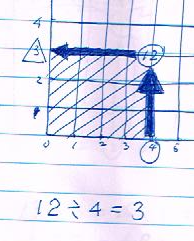
\includegraphics[width=0.3\textwidth]{division_res/division}
         \caption{用乘法表计算$12\div4$}
         \label{img_division}
    \end{figure}
    
大家试试用乘法表计算$48\div6$。如果你的乘法表只有下半部分,会遇到什么问题呢?又该如何解决呢?

\section{分配律}

乘法有分配律,那么除法呢?以铺砖为例,如果每行需要3块方砖,第一次运来12块砖,可以铺4行,第二次运来6块砖,可以铺2行,总共可以铺6行。如果这两批砖一次运到,可以普几行呢?还是6行。用数学式子表达 $12\div3 + 6\div3 = 6\frac{18}{3} = 6$ 所以$(12+6)\div 3 = 12\div3 + 6\div3$。也就是说,除法也有分配律。

除法有交换律么?

和乘法一样,分配律可以帮助我们把一个复杂的问题化解成相对简单的几个问题。 比如,$126\div3 = (12\times10+6)\div3 = 12\times10\div3 + 6\div3 = 10\times12\div3 + 2 = 42$ 想一想,如果把126写成$1\times100+2\times10+6$呢?

\section{整除和余数}

刚才计算了$12\times4$,再来算一个$12\times3$巩固一下。

那么$13\div3$等于多少?回到乘法表(图\ref{img_remainder})用刚才的方法,从横轴找到3,然后向上走,找不到13。找到12之后,下一个就是15。在这种情况下,我们说,13不能被4整除。

\begin{figure}[h]
     \center
     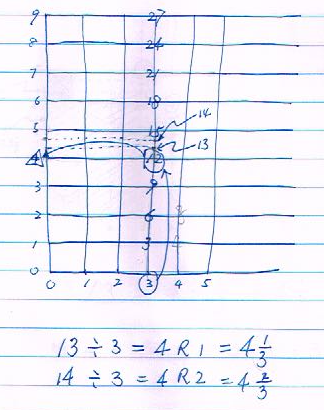
\includegraphics[width=0.8\textwidth]{division_res/remainder}
     \caption{}
     \label{img_remainder}
\end{figure}

我们注意到$13 = 12 + 1$,而$12=3\times4$,所以$13 = 3\times4 + 1$。所以,$13\div3$的结果就记录成$4R1$。这里第二个数称为余数(remainder),它的意义是,如果13里面拿掉这个余数1,它就可以被3整除,商为4。

15可以被3整除么?16呢?17呢?余数只能是1和2。假设有一个数,被3除,余数是3,商是6,那么,如果商是7,余数即为0,也就是说,这个数可以被3整除。如果余数大于3,我们可以从余数里拿掉一个3,把商加1,再拿掉一个3,再把商加1,直到余数是1或者2。试着用乘法表解释一下这个推理过程。(图\ref{img_remainder})

再回忆一下十进制的概念:$87 = 8\times10+7$。十位上的8,其实就是$87\div10$的商,个位上的7就是余数。

\section{分数} 虽然我们引入了余数的概念,但这并没有回答最初的问题。$13\div4$的目的是,给定13块方砖,每行铺3块,一共能铺几行。如图\ref{img_remainder}中所示,在铺满4行之后,还剩余1块。这剩余的1块,显然不够铺满第五行。所以,我们至少可以说,行数应在4和5 之间。这就给行数确定了一个更小的范围。有的时候,能够很快的估计出结果的大致范围比花很多精力计算准确结果更有实际意义。

这剩余的1块砖,当然只能满足铺满下一行所需3块砖中的一块,我们把这种情况记为3分之1。这种记法需要两个数:剩余的砖数1,和所需的砖数3。我们可以说,剩下的这块砖可以铺满3分之1行。结合已经铺满的前4行,我们的结果是13块砖,每行3块,可以铺满4又3分之1行(“又”就是加的意思)。

3分之1一般记为$\frac{1}{3}$。这个记法和1除以3一样,它的意义也是一样的。回忆以下,1除以3的意思不就是总共有1块砖,每行需3块,可以铺几行的意思么?所以,我们的结果可以记成$4\frac{1}{3}$。
虽然13不能被3整除,前面讲的用乘法表算除法的方法也是可以使用的。首先,还是从横轴的3向上走,虽然不能找到13,但是我们可以在12和15中间找到一个点作为13。这个点应该选在哪里能?它和12的距离,应该是它和15的距离的一半。然后,我们向左转,走到纵轴,就会停在4和5之间。这就是我们的结果。这个结果对应的点与4的距离,是它与5的距离的一半(想想为什么)。换句话说,如果我们把4到5之间的距离等分成3份,$13\div3$的结果就是4再加上这3份中的1份。这额外的一份就是$1\div3$(图\ref{img_remainder})。为什么这样说?因为从4到5需要走3步,而$13\div3$的结果只走完了其中的1步。

我们刚才,完全从形式出发,把乘法表从整除拓展到了不能整除的情况。在数学上,有种技术叫做延拓(continuation),是这种思想的进一步发展。

作为巩固,试着算一下$14\div4$。结果是$3\frac{1}{2}$还是$3\frac{2}{4}$呢?画图解释一下。

\section{除法的应用}
\subsection{可用除法表示的各种关系}

前面的例子告诉我们,如果行数$\times$每行砖数 = 总砖数,那么
行数 = 总砖数$\div$ 每行砖数。注意到我们需要重复同样的每行3块砖,除法帮助我们得到了重复的次数。同样的,能不能得出一个类似结论, 每行砖数 = 总砖数$\div$行数?也就是说,通过重复的次数(行数),除法可以得到每次需要的砖数。尝试用交换律解释一下。 回想面积的定义,上面的关系也可以写成 高 = 面积$\div$宽, 宽 = 面积$\div$高。

类似的,既然
人数$\times$每人分得糖数=总糖数,
那么 
人数 = 总糖数$\div$每人分得糖数,或者 每人分得糖数 = 总糖数$\div$人数。

\subsection{方程与维度}

迄今为止,我们都是在试图通过已知条件,计算未知。换句话说,等号左边是未知数,等号右边告诉我们如何通过已知条件来计算。这些用等号连接的表达式叫做方程(Equation)。方程不仅给出了如何用右边的已知计算左边的位置,更重要的是,方程建立了数字之间的等价关系。

比如,面积 = 高$\times$ 宽, 就是建立了高、宽和面积之间的关系。宽 = 面积$\div$高 也建立了这三者之间的关系。由于这两个方程描述的是同样的事实(铺砖),他们实际上是一样的,确切的说,是等价的。换句话说,我们只需要这两个方程之一。实践上,我们也是这样做的,从乘法出发,把除法建立在乘法的基础之上。以后我们会更进一步讨论,如何证明、使用这样的等价关系。

现在,我们只需要理解,方程建立了不同量值之间的关系。再观察一下乘法表(图\ref{img_dof}),如果我们没有任何限制条件,可以选择任意两个数计算他们的乘积。如果是铺砖,可以选择任意行数和每行砖数;如果是面积,可以选择任意的宽或者高。为了不被具体的问题限制,我们把这两个数称为$X$和$Y$,并且约定$X$对应横轴上的数字,$Y$对应纵轴上的数字。由于我们可以自由选择两个数字,我们就有“两个自由度”(two degrees of freedom)。根据我们选择的这两个数字,我们计算乘法时,就可能会落到乘法表上的任意一个点。

\begin{figure}[h]
     \center
     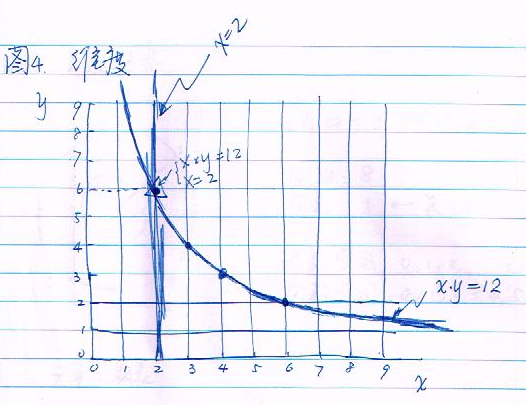
\includegraphics[width=0.8\textwidth]{division_res/dof}
     \caption{方程与自由度}
     \label{img_dof}
\end{figure}

介绍除法时,我们引入了总砖数这个限制条件,比如,总砖数为12。注意到总砖数=行数$\times$每行砖数。这样的条件实际上限制了行数和每行砖数的乘积。如果不考虑具体问题,我们相当于引入了一个限制条件,规定了两个数的乘积为12。这个关系,用方程表示就是$X\times Y = 12$。在图四中,我们再次画出了满足这个条件的点所连成的线(双曲线)。有了这个条件,我们就不能完全自由选择$X$和$Y$的值。符合要求的$X$和$Y$对应的乘积必然在这条双曲线上。如果我们进一步选择$Y=3$,那么$X=12\div3=4$,也成为一个定数。如果我们选择$Y=2$,那么$X=12\div2=6$,也成为一个定数。换句话说,如果$Y$确定了,$X$也就确定了,这样,我们就只剩一个自由度。自由度的减少是由于我们引入了一个限制条件(方程)。如果我们在要求$X\times Y = 12$的同时,还要求$X=2$,那么$Y$必然等于6,也就是说,我们没有任何自由度来选择$X$和$Y$的值,最初的两个自由度,就被$X\times Y = 12$和$X=2$这两个方程去除了。

我们可以形象的描述这个自由度消失的过程。起初,整个乘法表都是可供我们选择的(两个自由度),一旦我们指定$X\times Y = 12$,我们就被限制在那条双曲线上(一个自由度),当进一步指定$X=2$,我们就被限制在三角形圈定的那个点(无自由度)。这个过程又提示了另一种用乘法表计算除法的过程:如果计算$12\div2$,一只手指在双曲线上运动,另一只手指从横轴的2开始向上走,两者碰头时,再向左找到纵轴对应的点,即为商。回忆一下我们前面讲的除法的计算过程,也体现了类似的从两个自由度,到一个自由度,最好没有自由度的过程。

手指碰头的过程,实际是两条线——双曲线和直线——相交的过程。$X\times Y = 12$这个方程,对应的是双曲线;$X = 2$这个方程,对应的是直线(图\ref{img_dof})。用除法计算$12\div2$的过程,就是找这两条线交点的过程。

你能用类似的方法计算$24\div6$和$50\div8$么?

\subsection{余数的意义——幸运转盘} 大家玩过幸运转盘,如果一共有12个位置,而指针转过了23个位置,你的奖品和指针转过35个位置就是一样的。这是因为23$\div$12和35$\div$12的余数都是11。在玩幸运转盘时,余数是取决定作用的,转过了多少圈并不重要, 见图\ref{img_wheel}。 

    很多实际问题都有这个特点:余数更重要。往往这和周期性的现象相联系。比如,如果今天是周四,7天过后还是周四,14天过后也还是周四,那么一年365天以后呢?另一个有名的例子是元素周期表,科学家们发现,化学元素的性质也在很大程度上由价电子数决定,而这个价电子数就是总电子数除以8的余数。
\begin{figure}[h]
     \center
     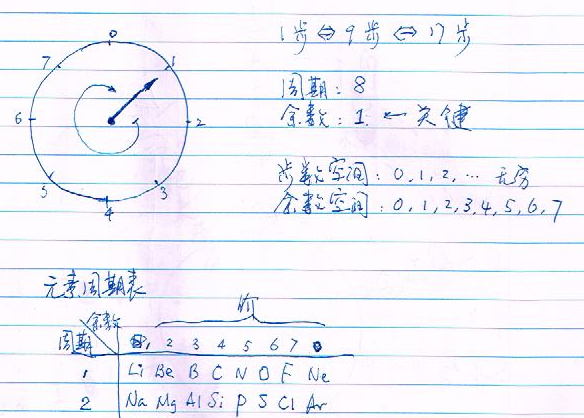
\includegraphics[width=0.6\textwidth]{division_res/wheel}
     \caption{余数的意义。幸运转盘和元素周期表。}
     \label{img_wheel}
\end{figure}

\subsection{平均值} 
除法可以帮助我们计算平均值。比如我们想要把150块糖分给10位小朋友,如果每人分的糖数一定,那么每人可以分得$150\div10=15$块。更多的时候,我们用平均值来描述一些更复杂的情况。

\begin{figure}[h]
     \center
     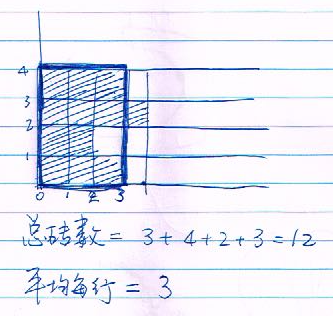
\includegraphics[width=0.6\textwidth]{division_res/average}
     \caption{平均值}
     \label{img_average}
\end{figure}

还以铺砖为例,如果每行所用砖数并不一样,如图\ref{img_average}所示,第一行至第四行个用了3,2,4,3块砖,一共12块。为了方便的描述这种情况,我们说,每行平均用了3块砖。这样,只用一个平均值(3)就可以大致代替每行的砖数。虽然我们忽略了一些细节,但是方便了很多。更重要的是,平均值可以帮助我们描述铺砖这个问题里面的很多有用信息。如果我们关心的是使用的总砖数,又不想繁琐的记录每行具体有多少砖,那就可以假想一种每行砖数都一样的情况,但是,这个假想的情况应该使用同样的总砖数和行数。也就是说,
\begin{itemize}
    \item 假想情况下每行砖数 $\times$ 行数 = 假想情况下总砖数 = 实际情况下总砖数
    \item 假想情况下每行砖数 = (第一行砖数 + 第二行砖数 + 第三行砖数 + 第四行砖数)$\div$ 行数
\end{itemize}


这个假想情况下的每行砖数就是平均每行的砖数。

有时,我们看到一大片砖,想要知道一共用了多少块。如果每行每行的数,会很费事。那就可以先数几行,计算一下平均每行有多少块砖,再数一下一共多少行,就可以估计一共多少块砖了。你觉得需要先数多少行计算平均值才“保险”呢?等你学到统计学,就知道答案了。

平均值的定义不是唯一的。还是铺砖为例,如果我们每行用两种不同价格的砖之一,每行的花费自然也不同。为了大致描述每行的花费,我们还是假想一种每行花费一样的情况,而保证行数和总花费一致,那么

假想情况下每行花费 = 总花费 $\div$ 行数 = (第一行砖数$\times$第一行砖价 + 第二行砖数$\times$第二行砖价 + 第三行砖数$\times$第三行砖价 + 第四行砖数$\times$第四行砖价) $\div$ 行数

有人把这种平均值叫做加权平均值(weighted average),每行的砖价即为“权”(weight)。实际上,这也是平均值的一种,其背后的想法是一致的。

计算平均值,要记住它的目的是用一个值(平均值),概括更加复杂的实际情况,同时保证我们所关心的量(比如总花费)不受影响。一个非常典型的例子是平均速度。假设从家到学校要走两站路,每站之间距离相等,都是1公里,但是汽车在每站之间的速度不一样。从第一站到第二站,速度为20公里/小时,从第二站到第三站,速度为18公里/小时,那么,平均速度为多少?这里,我们想要引入平均速度,用这一个数值,代替各个路段的具体速度,那么什么量应该不受影响呢?通常,大家关心路上所耗时间,如果我们用一个单一的平均速度计算路上耗时,其结果应该和分别考虑各路段具体速度所得结果一致。

\begin{itemize}
    \item 使用平均速度:路上耗时 = 2/平均速度
    \item 使用各路段速度:路上耗时=1/20 + 1/18
\end{itemize}
     
     这两种情况应该得到同样结果,

2/平均速度 = 1/20 + 1/18 

    那么,平均速度应该这样定义,
    
平均速度 = 2/(1/20+1/18) 

人们也把这类平均值称为调和平均值。

\subsection{天干地支}
\begin{figure}[h]
     \center
     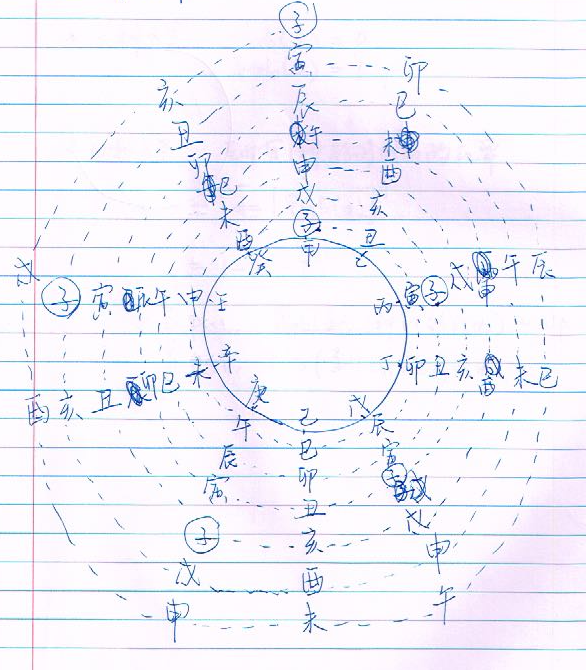
\includegraphics[width=0.6\textwidth]{division_res/ganzhi}
     \caption{}
     \label{img_ganzhi}
\end{figure}




